\begin{center}
    \textsc{\Large\textbf{Slope of a line}}
\end{center}
    \begin{center}
        \begin{tikzpicture}
            \tzaxes(-2, -1.5)(7, 4){$x$}{$y$}
            \tzline"L1"(0, 0)(6, 4){$L_1(x)$}[ar]
            \tzline"L2"(0, 0)(6, 2){$L_2(x)$}[ar]
            \tzline[dashed]"DL"(4, 0)(4, 4)
            \tzXpoint{DL}{L1}(X1)
            \tzXpoint{DL}{L2}(X2)
            \tzdot*(X1)
            \tzdot*(X2)
            \tzline[|<->|]<0, -0.5>(0, 0)(4, 0){$\Delta x$}[mb]
            \tzline[|<->|]<0.5, 0>(4, 0)(X2){$\Delta y_2$}[mr]
            \tzline[|<->|]<1.5, 0>(4, 0)(X1){$\Delta y_1$}[mr]
        \end{tikzpicture}
    \end{center}
    \begin{quote}
        \textit{
            The slope of a line is a measure of its steepness and direction, and it can be interpreted as the rate of change of the line. It is calculated as the ratio of the vertical change to the horizontal change between two distinct points on the line.\\[2mm]
            In the above diagram $L_1$ and $L_2$ are two lines, $\Delta x$ is the horizontal change, and $\Delta y_1$ and $\Delta y_2$ are the vertical changes of the lines $L_1$ and $L_2$ respectively.\\[2mm]
            As you can see $\Delta y_1 > \Delta y_2$ and $\Delta x$ is the same for both the lines. Therefore, the slope of the line $L_1$ is greater than the slope of the line $L_2$.\\[2mm]
            Here, for both the lines $L_1$ and $L_2$, for $\Delta x > 0$, $\Delta y_1 \textit{ and } \Delta y_2$ are positive. Therefore, the slope of the line is positive.
        }
    \end{quote}
    \begin{itemize}
        \item But slope can be negative if $\Delta y < 0$ for $\Delta x > 0$.
            \begin{center}
                \begin{tikzpicture}
                    \tzaxes(-2, -1)(7, 4){$x$}{$y$}
                    \tzcoors*(1,1)(A)(1,2)(B)(3,1)(C);
                    \tzLFn(B)(C)[-1:5]
                    \tzline[dashed](A)(B)
                    \tzline[dashed](A)(C)
                    \tzline[|<->|]<-0.25, 0>(A)(B){$\Delta y$}[ml]
                    \tzline[|<->|]<0, -0.25>(A)(C){$\Delta x$}[mb]
                \end{tikzpicture}
            \end{center}

        \item Slope can be zero if $\Delta y = 0$ for all $\Delta x \neq 0$.
            \begin{center}
                \begin{tikzpicture}
                    \tzaxes(-2, -1)(7, 3.5){$x$}{$y$}
                    \tzcoors*(1, 2)(A)(3, 2)(B);
                    \tzLFn(A)(B)[-1:5]
                    \tzline[|<->|]<0, -0.25>(A)(B){$\Delta x$}[mb]
                \end{tikzpicture}
            \end{center}

        \item Slope can be undefined if $\Delta x = 0$\\
            In this case, the line is vertical, meaning the slope tends to infinity. This situation violates the definition of slope because the slope is the ratio of the vertical change to the horizontal change. However, when the horizontal change is zero but the vertical change is not zero, this ratio becomes undefined.
            \begin{center}
                \begin{tikzpicture}
                    \tzaxes(-2, -1)(7, 4){$x$}{$y$}
                    \tzcoors*(1, 1)(A)(1, 3)(B);
                    % \tzLFn(A)(B)[-1:5]
                    \tzline($(A)+(0, -1.5)$)($(B)+(0, 1)$)
                    \tzline[|<->|]<-0.25, 0>(A)(B){$\Delta y$}[ml]
                \end{tikzpicture}
            \end{center}
    \end{itemize}
    % \pagebreak
\vspace*{10mm}
    \begin{center}
        \textsc{Slope of a line passing through two points $P(x_1, y_1)$ and $Q(x_2, y_2)$}\\[10mm]
        \begin{tikzpicture}
            \tzaxes(-2, -1)(7, 4){$x$}{$y$}
            \tzcoors*(4,1)(A)(1,1)(B){$P(x_1, y_1)$}[al](4,3)(C){$Q(x_2, y_2)$}[al];
            \tzLFn(B)(C)[-1:5]
            \tzline[dashed](A)(B)
            \tzline[dashed](A)(C)
            \tzline[|<->|]<0, -0.5>(A)(B){$\Delta x$}[mb]
            \tzline[|<->|]<0.5, 0>(A)(C){$\Delta y$}[mr]
            \tzanglemark(A)(B)(C){$\theta$}(15pt)
        \end{tikzpicture}
    \end{center}
    \begin{align*}
        \intertext{Slope of a line passing through two points $P(x_1, y_1)$ and $Q(x_2, y_2)$:}
        \textit{Slope(m) } &= \frac{\Delta y}{\Delta x} \\
        \intertext{From the above diagram,}
        \tan \theta &= \frac{\Delta y}{\Delta x} \\
        \intertext{Therefore,}
        \Aboxed{m &= \tan \theta = \frac{y_2 - y_1}{x_2 - x_1}}
        \intertext{Be careful, $\theta$ is the angle between the line and the positive x-axis in anti-clockwise direction.}
    \end{align*}